\documentclass[12pt, 
hyperref={colorlinks=true, linkcolor=blue, urlcolor=cyan}]{beamer}
\usetheme{default} 

\setbeamertemplate{navigation symbols}{} %gets rid of navigation symbols
\setbeamertemplate{footline}{} %gets rid of bottom navigation bars
\setbeamertemplate{footline}[page number]{} %use this for page numbers

\setbeamertemplate{itemize items}[circle] %round bullet points
\setlength\parskip{10pt} % white space between paragraphs

\usepackage{wrapfig}
\usepackage{subfig}
\usepackage{setspace}
\usepackage{enumerate}
\usepackage{graphicx}
\usepackage{amsmath}
\usepackage{amsfonts}
\usepackage{amssymb}
\usepackage{amsthm}
\usepackage[UKenglish]{isodate}
\usepackage{verbatim}
\cleanlookdateon

% the preamble
\title{BIOST 311: \\ Regression Methods for the Health Sciences}
\author{Kelsey Grinde and Brian Williamson}
\institute{UW Biostatistics}
\date{Spring 2018}

\begin{document}
% title slide
\begin{frame}
\titlepage\thispagestyle{empty}
\end{frame}

% make it 1.something
\setbeamertemplate{footline}{%
  \raisebox{5pt}{\makebox[\paperwidth]{\makebox[120pt]{\scriptsize Last updated \today}\hfill\makebox[10pt]{\scriptsize 1.\insertframenumber~~}}}}  \newcounter{chap1}{\value{1}}
\setcounter{framenumber}{\value{chap1}}

\begin{frame}
\frametitle{CHAPTER 1: LINEAR REGRESSION}
By the end of Chapter 1, you should be able to: \vspace{-0.3cm}

\begin{itemize}
\item Formulate a regression model, given a scientific or statitical question
\item Interpret the coefficients for a (simple or multiple) linear regression model
\item Interpret confidence intervals and p-values for linear regression coefficients
\item Classify variables according to their role in a linear regression model (e.g., outcome, predictor, potential confounder, effect modifier, precision variable)
\item Use \texttt{R} to fit a linear regression model (and know where in the output to look for the information we need to interpret results)
\item Create graphs to support your linear regression analysis
\end{itemize}

\end{frame}

\section{Simple Linear Regression}
\begin{frame}
\frametitle{SECTION 1: SIMPLE LINEAR REGRESSION}

\center 
\color{red} \begin{large} $y = a + bx$ \end{large} 

\vspace{-0.2cm} 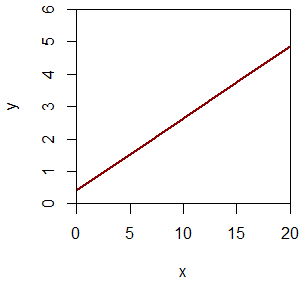
\includegraphics{./plots/plot_y_vs_x}

\end{frame}

\begin{frame}
\frametitle{Determining the slope and intercept of a line}

\center
\begin{large} \color{red} $y = a + bx$ \end{large} \color{black}: \textit{What is a? What is b?}

\vspace{-0.2cm} 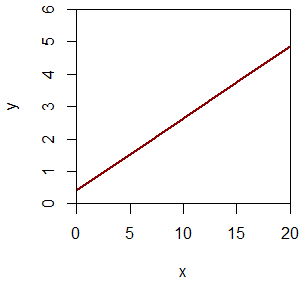
\includegraphics{./plots/plot_y_vs_x} % practice on this example, write interpretation on white board (to come back to)

\end{frame}

\begin{frame}
\frametitle{Simple linear regression}

\begin{center} 
 \color{red} $E[Y|X] = \beta_0 + \beta_1 X$ \color{black}
\end{center} \vspace{-0.3cm}

\begin{small} \textit{Let's take our data, and fit the ``best" line through it. That line models the average outcome $Y$ (e.g., FEV), given the predictor $X$ (e.g., age), as a linear function of $X$ (e.g., age).} \end{small}

\center
\vspace{-0.3cm} \center 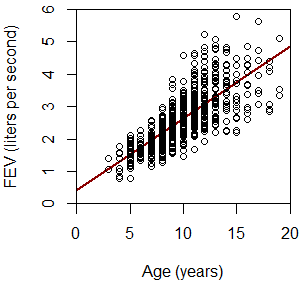
\includegraphics[height=0.65\textheight]{./plots/plot_fev_vs_age}

\end{frame}

% explain linear regression notation
\begin{frame}
\frametitle{Simple linear regression: notation and terminology}
$$\color{blue} E[Y|X] \color{black} = \color{orange} \beta_0 \color{black} + \color{red} \beta_1 \color{yellow} \ X$$ \vspace{-0.6cm}

\color{blue}The average of the response, given the value of the predictor, \color{black} is \color{orange} the intercept \color{black} plus \color{red} the slope \color{black} times \color{yellow} the value of the predictor.\color{black} \pause

\vspace{-0.2cm}
\begin{itemize}
\item $Y$ = outcome, response
\item $X$ = exposure, predictor \pause
\item $E[Y] =$ expected value =  mean of $y$ in the population \pause
\item $E[Y|X]$ = conditional expectation = population mean of $Y$, given information about $X$	\pause
\item Examples: $Y$ is height, $X = 1$ if female and $0$ if male
	\begin{itemize}
	\item $E[Y]$ = 67.1" (the average height in the population)
	\item $E[Y|X = 0]$ = 69.7" (the average height of males)
	\item $E[Y|X = 1]$ = 64.6" (the average height of females)
	\end{itemize}
\end{itemize}
\end{frame}

% interpreting slope and intercept
\begin{frame}
\frametitle{Simple linear regression: interpretation}

The \textit{coefficients} ($\beta_0$,$\beta_1$) in our simple linear regression model $E[Y|X] = \beta_0 + \beta_1 X$ often have useful interpretations.

Let's start with the intercept, $\beta_0$: \textit{how would you interpret this coefficient?} \vspace{-0.3cm}
\begin{itemize}
\item[] (Hint: think about how we interpret $a$ in $y=a+bx$)\pause 
\item[] \color{blue} $\beta_0$ is the mean value of $Y$ among subjects with $X = 0$ \color{black}
\end{itemize}

And now the slope, $\beta_1$: \textit{how would you interpret this coefficient?} \vspace{-0.3cm}
\begin{itemize}
\item[] (Hint: think about how we interpret $b$ in $y=a+bx$) \pause
\item[] \color{blue} $\beta_1$ is the difference in mean value of $Y$ comparing two groups that differ in $X$ by one unit \color{black}
\end{itemize}

\end{frame}

% practice: interpreting intercepts
\begin{frame}
\frametitle{Practice: interpreting intercepts in context}

\begin{center} $E[\text{FEV} | \text{age}] = 0.43 + 0.22 \times \text{age}$ \end{center} 

Which of these is correct? \vspace{-0.3cm}
\begin{enumerate}
\item A newborn child will have FEV equal to 0.43 liters per second
\item Among all newborn children, the average FEV is 0.43 liters per second
\end{enumerate} \pause

\textit{Does this interpretation make sense  scientifically?} \\ \pause  % Yes, age = 0 <--> birth
\textit{What if I replaced age with height in the formula above?} \\ \pause % No, height = 0 <-- DNE
\textit{What if we did this study on adults (ages 40--60), and got the same intercept? Would you trust the intercept?} %% No! Be careful not to extrapolate too far beyond range of data

\end{frame}

% practice: interpreting slopes
\begin{frame}
\frametitle{Practice: interpreting slopes in context}

\begin{center} $E[\text{FEV} | \text{age}] = 0.43 + 0.22 \times \text{age}$ \end{center} 

\textit{What is the difference between these two interpretations?} \vspace{-0.3cm}
\begin{itemize}
\item For every one year increase in age, average FEV increases by 0.22 liters per second
\item Comparing two groups of children that differ in age by one year, the difference in average FEV will be 0.22 liters per second, with higher average FEV in the older of the two groups
\end{itemize} \pause

\textit{Which do you think is correct?} \pause (Hint: this was an observational study)

% give a couple examples, some with interpretations that are ``too causal"
\end{frame}

% why do we care about the slope?
\begin{frame}
\frametitle{Why do we care about the slope?}

\begin{small} \textit{In which example(s) is there no association between FEV and age?} \vspace{-0.2cm} \end{small}

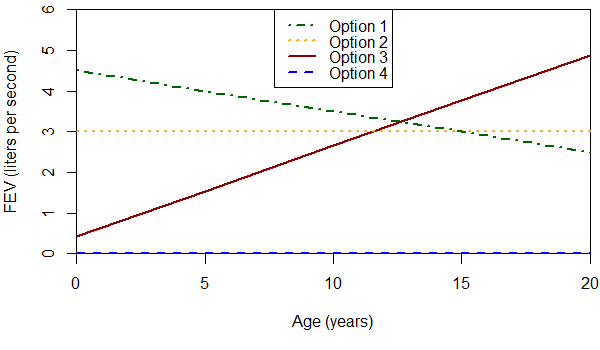
\includegraphics[width=\textwidth]{./plots/association}
\pause
\textit{What is the slope in those cases?}
\end{frame}

\begin{frame}
\frametitle{Why do we care about the slope?}

When $\beta_1 = 0$: there is no association between $X$ \& $Y$

When $\beta_1 > 0$: there is a positive association between $X$ \& $Y$

When $\beta_1 < 0$: there is a negative association between $X$ \& $Y$

So... if our scientific question is \textit{is there an association between FEV and age?}, we can use linear regression to answer this question, by checking whether $\beta_1$ in the model $E[FEV|age] = \beta_0 + \beta_1 \times age$ is 0!

\end{frame} 


% math explaining slope interpretation
\begin{frame}
\frametitle{Interpreting slopes: mathematical explanation}

For a regression model $E[Y|X] = \beta_0 + \beta_1 X$, we interpret the slope $\beta_1$ as the difference in mean value of $Y$ for two groups differing in $X$ by one unit.

Why is this true?
\begin{itemize}
\item $E[Y|X = x] = \beta_0 + \beta_1 x$ \pause
\item $E[Y|X = (x+1)] = \beta_0 + \beta_1(x+1) = \beta_0 + \beta_1 x + \beta_1$ \pause
\item $E[Y|X = (x+1)] - E[Y|X = x] = \beta_1$ \pause
\end{itemize}

\end{frame}

\begin{frame}
\frametitle{What's next?}

\begin{itemize}
\item Confidence intervals and hypothesis tests for regression parameters
\item What it means to find the line of ``best" fit
\item Using \texttt{R} to fit linear regression models 
\end{itemize}

\end{frame}



% comment out mutliple linear regression section %%%%%%%%%%%%%%%%%%%%%%%%%%%%
\begin{comment} 
\section{Multiple Linear Regression}
\begin{frame}
\frametitle{SECTION 2: MULTIPLE LINEAR REGRESSION}
By the end of Section 2, you should be able to:

\begin{itemize}
\item Identify potential variables that \textcolor{red}{confound} the association between the predictor of interest and the outcome, and
\item describe \textbf{why} you will adjust for these variables in a regression analysis.
\item Identify potential variables that \textcolor{blue}{modify} the association between the predictor of interest and the outcome, and  
\item describe \textbf{how} you will test for  differential effects.
\item Identify potential variables that help \textcolor{green}{reduce the variability} of our estimates.
\item \textbf{Interpret} parameters in a multiple linear regression model.
\item \textbf{Fit} multiple linear regression models in \texttt{R}, and
\item \textbf{interpret} the output to perform hypothesis tests.
\end{itemize}

\end{frame}

\begin{frame}
\frametitle{Multiple regression: motivation}

So far, we have considered the relationship between the outcome, $Y$, and a \textcolor{green}{single} predictor of interest, $X$.

However, there may be other variables that influence the association between our predictor of interest and the outcome, by:
\begin{itemize}
\item \textcolor{red}{confounding} the association 
\item \textcolor{blue}{modifying} the association
\item providing information that \textcolor{green}{reduces the variability} of our estimates
\end{itemize} 
\end{frame}

\begin{frame}
\frametitle{Multiple regression: motivation}
What do you think the relationship is between $X_1$ and $Y$?

\vspace{-0.3cm}
\centering
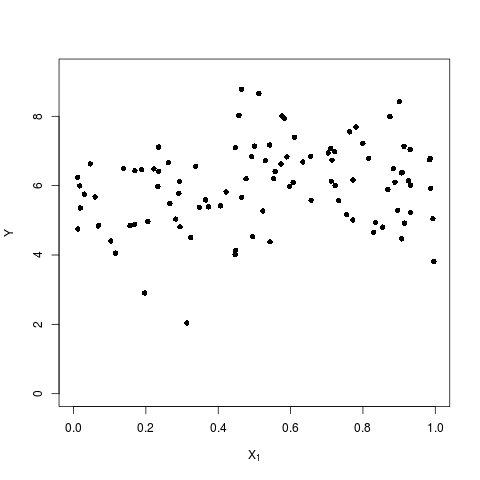
\includegraphics[width = 0.7\textwidth]{./plots/confounding_simple.png}
\end{frame}

\begin{frame}
\frametitle{Multiple regression: motivation}
What do you think the relationship is between $X_1$ and $Y$?

\vspace{-0.3cm}

\centering
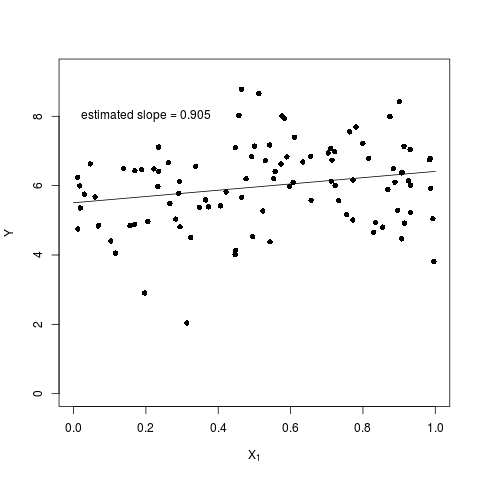
\includegraphics[width = 0.7\textwidth]{./plots/confounding_simple_with_line.png}
\end{frame}

\begin{frame}
\frametitle{Multiple regression: motivation}
How about now?

\vspace{-0.3cm}
\centering
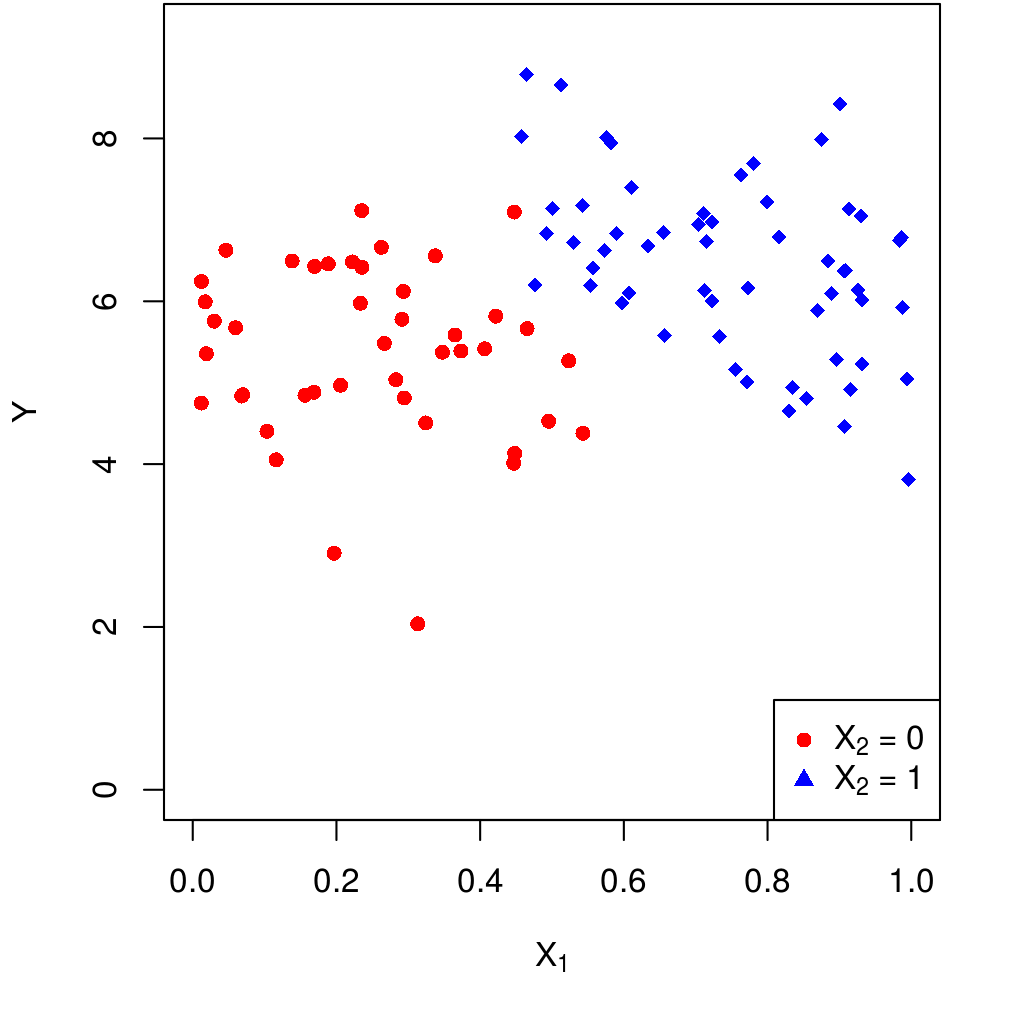
\includegraphics[width = 0.7\textwidth]{./plots/confounding_colored.png}
\end{frame}

\begin{frame}
\frametitle{Multiple regression: motivation}
How about now?

\vspace{-0.3cm}
\centering
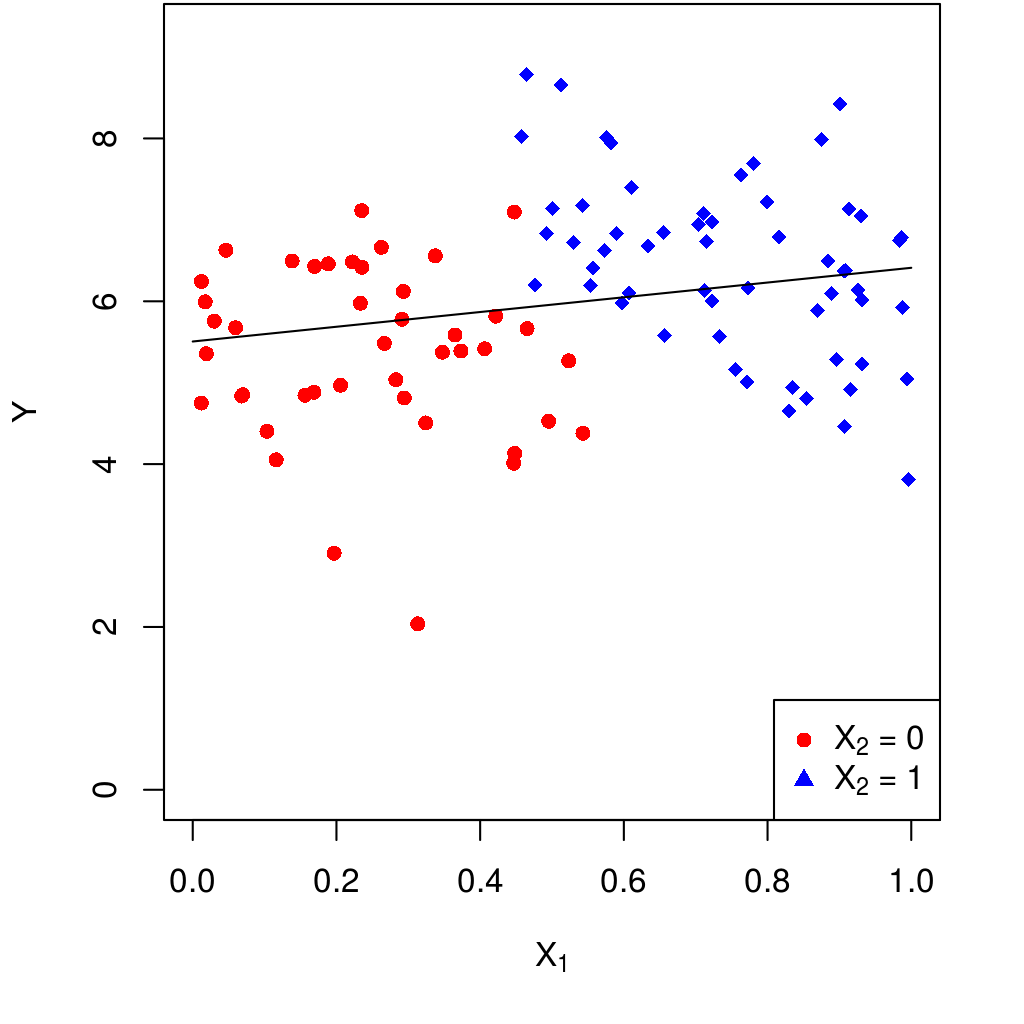
\includegraphics[width = 0.7\textwidth]{./plots/confounding_colored_with_simple_line.png}
\end{frame}

\begin{frame}
\frametitle{Multiple regression: motivation}
How about now?

\vspace{-0.3cm}
\centering
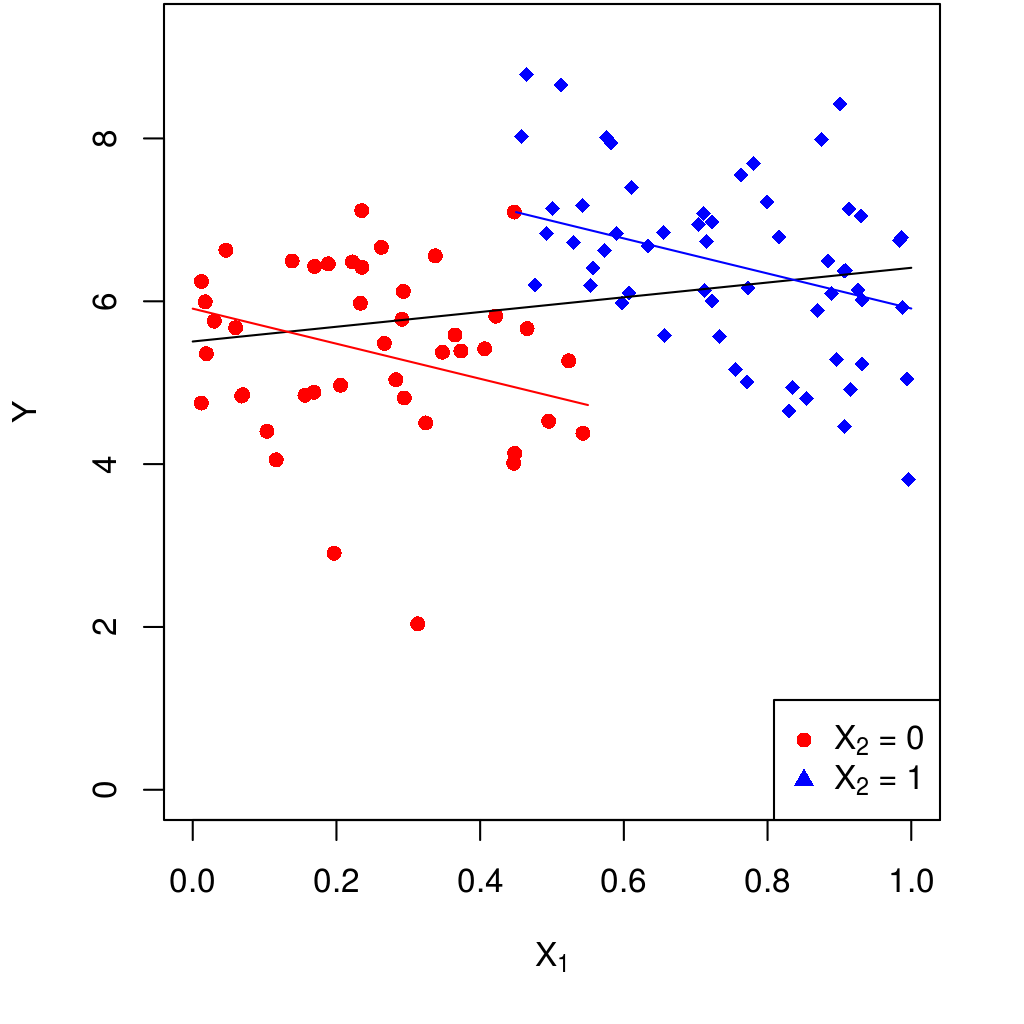
\includegraphics[width = 0.7\textwidth]{./plots/confounding_colored_with_lines.png}
\end{frame}

\begin{frame}
\frametitle{Multiple regression: notation}
\end{frame}

\begin{frame}
\frametitle{Multiple regression: FEV}
\end{frame}


\section{Wrapping up}
\begin{frame}
\frametitle{SECTION 3: WRAPPING UP}
\end{frame}
\end{comment} % end comment block

\end{document}
